\section{Auswertung}
\label{sec:auswertung}

Im Folgenden wird die gemessene Magnetfeldstärke für verschiedene
Tiefen der Hall-Sonde in den Elektromagneten visualisiert, sowie die
effektive Masse von Elektronen in GaAs bestimmt.
Dafür wird der Faraday-Rotationswinkel in hochreinen GaAs bestimmt, sodass
das Einwirken der gebundenen Elektronen in GaAs auf den Rotationswinkel bekannt ist.
Weiterhin werden die Faraday-Rotationswinkel in zwei dotierten Proben
gemessen, sodass der Einfluss von freien Eletronen auf den Rotationswinkel
ermittelt werden können.
Die Auswertung ist mit Hilfe der \textit{python}-Pakete
\textit{scipy\_curvefit} und \textit{numpy} bewerkstelligt worden.
Konstanten wie die Elektronenmasse $m_e$ oder die dielektrische Konstante $\epsilon_0$
sind dem \textit{python}-Paket \textit{scipy\_constants} entnommen.

\subsection{Magnetfeld}

Die gemessenen Werte des $B$-Feldes sind in Abbildung~\ref{fig:B} dargestellt.
Auf eine Ausgleichrechnung für die Ermittlung von $B\ua{max}$ wird verzichtet,
da in dem Bereich um den Hochpunkt von $B(s)$ ausreichend viele Messpunkte vorliegen.
An der Stelle des maximalen Magnetfeldes wird die Probe eingesetzt.
Das maximale $B$-Feld ergibt sich zu
\begin{equation}
  \label{eqn:b_max}
  B\ua{max} = \SI{426}{\milli\tesla}.
\end{equation}
\vspace{-10pt}
\begin{figure}[h]
  \centering
  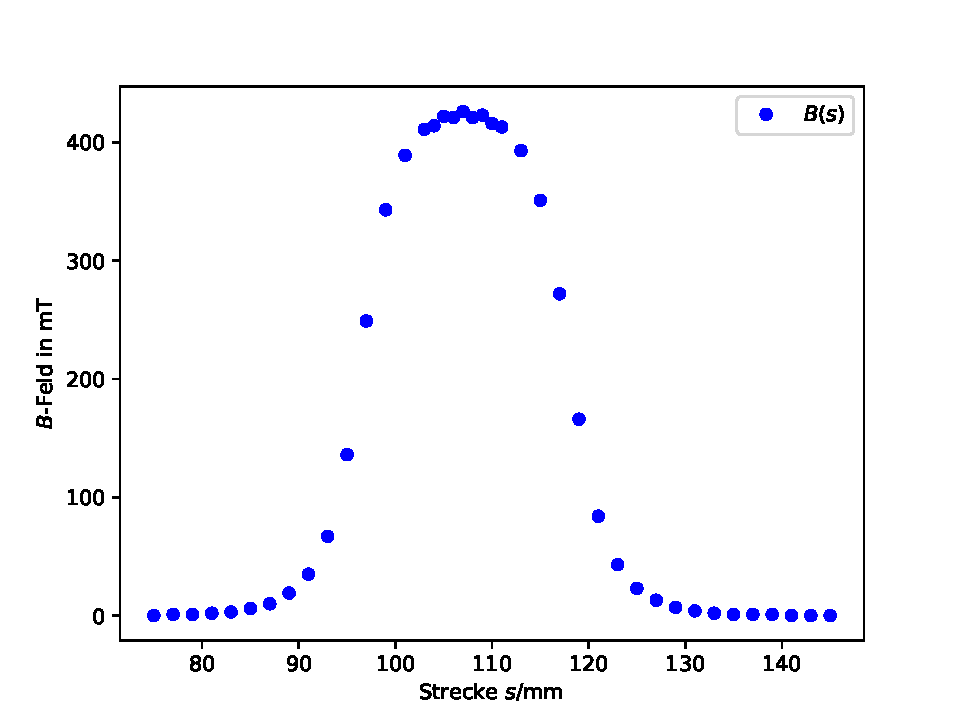
\includegraphics[width = 0.8\textwidth]{Plots/B.pdf}
  \caption{Gemessene Werte des Magnetfeldes $B$ für verschiedene Tiefen der Hall-Sonde.}
  \label{fig:B}
\end{figure}
\FloatBarrier
\subsection{Hochreines GaAs}
Der Faraday-Rotationswinkel der hochreine GaAs-Probe wird bestimmt, damit
dieser als Referenzwert für den Einfluss der gebundenen Kristallelektronen
bekannt ist. Die gemessenen Rotationswinkel $\theta$ sind in Abb.~\ref{fig:hr}
dargestellt.
Tabelle~\ref{tab:hr} enthält die aufgezeichneten Daten.
\begin{figure}[h]
  \centering
  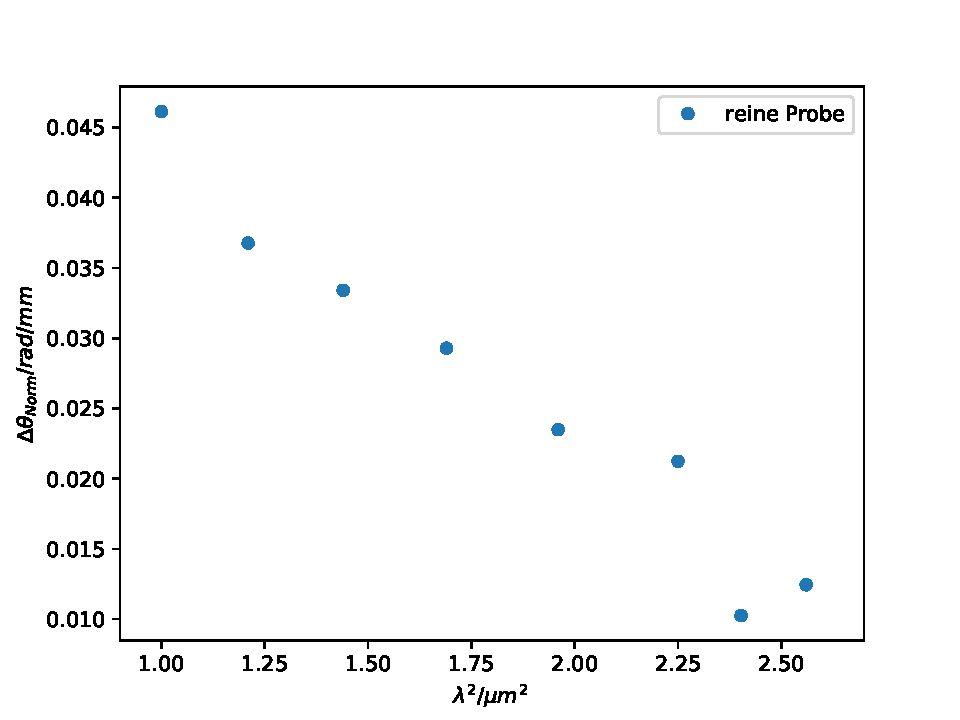
\includegraphics[width = 0.9\textwidth]{Plots/hr_GaAs.pdf}
  \caption{Normierte Faraday-Rotationswinkel der reinen GaAs Probe für verschiedene Wellenlängen $\lambda$.}
  \label{fig:hr}
\end{figure}

\begin{table}
\centering
\caption{Messwerte der reinen GaAs Probe, mit der Dicke $d = \SI{5.11}{\milli\meter}$. $\theta$ beschreibt den Faraday-Rotationswinkel
und $\theta_{\symup{Norm}}$ den über die Dicke normierten Faraday-Rotationswinkel.
$B_+$ und $B_-$ indizieren die Polung des Magnetfeldes.}
\label{tab:hr}
\begin{tabular}{S S S S S }
\toprule
{$\lambda / \si{\micro\meter}$} & {$\theta(B_+) / \si{\radian}$} & {$\theta(B_-) / \si{\radian}$}  & {$\theta / \si{\radian}$} & {$\theta\ua{Norm} / \si{\radian\per\mm}$}   \\
\midrule
1.00  & 2.40  & 2.87  & 0.236  & 0.046\\
1.10  & 2.43  & 2.80  & 0.188  & 0.037\\
1.20  & 2.45  & 2.79  & 0.171  & 0.033\\
1.30  & 2.48  & 2.78  & 0.150  & 0.029\\
1.40  & 2.53  & 2.77  & 0.120  & 0.023\\
1.50  & 2.51  & 2.73  & 0.109  & 0.021\\
1.55  & 2.73  & 2.83  & 0.052  & 0.010\\
1.60  & 2.71  & 2.83  & 0.064  & 0.012\\
\bottomrule
\end{tabular}
\end{table}

\FloatBarrier
\subsection{Dotiertes GaAs}
Im Folgenden wird die effektive Masse von freien Elektronen in GaAs kann bestimmt.
Die Tabellen~\ref{tab:probe1} und~\ref{tab:probe2}
enthalten die ermittelten Daten zu den dotierten Proben.
In Abbildung~\ref{fig:dot} sind die normierten und von dem
Referenzwinkel subtrahierten Faraday-Rotationswinkel
$\Delta\theta\ua{Norm}$
gegenüber $\lambda^2$ aufgetragen.
Die Ausgleichgeraden sind im Ursprung fixiert und haben somit
die Gestalt
\begin{equation}
  \label{eqn:fit}
  \Delta\theta\ua{Norm}\left(\lambda^2\right) = a\cdot\lambda^2
\end{equation}
Die Regressionsparameter zu~\eqref{eqn:fit} der einzelnen Proben
in Abb.~\ref{fig:dot} sind

Probe 1:
\begin{equation}
  \label{eqn:fit_1}
  a_1 = \SI{147(21)e-1}{\radian\per\nm^3}\\
\end{equation}
Probe 2:
\begin{equation}
  \label{eqn:fit_2}
  a_2 = \SI{210(25)e-1}{\radian\per\nm^3}.\\
\end{equation}
\begin{figure}
  \centering
  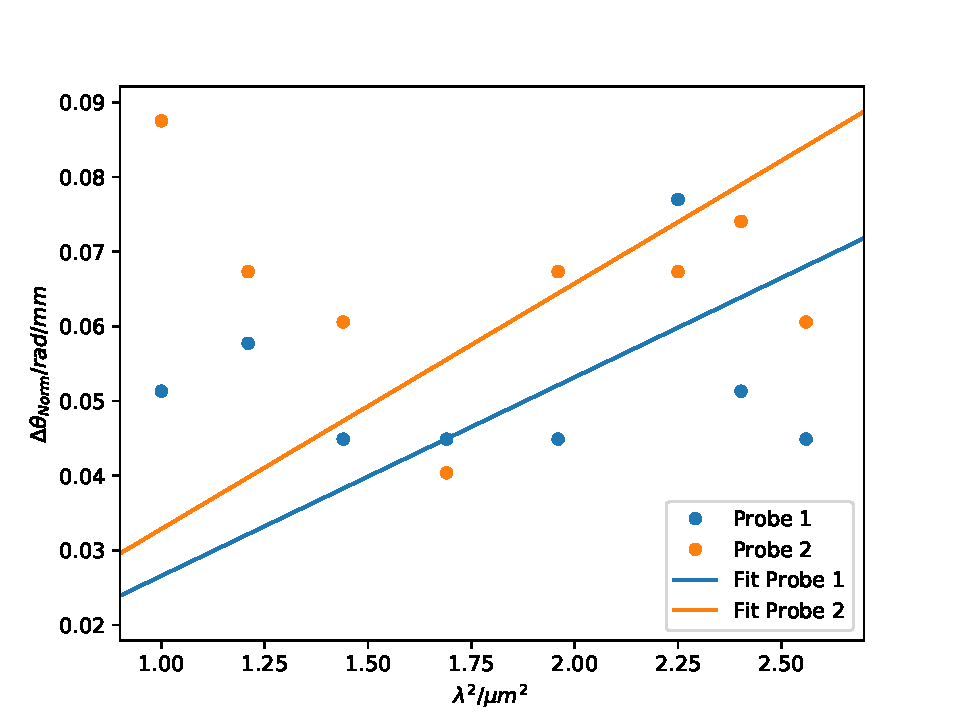
\includegraphics[width = \textwidth]{Plots/dotiert_GaAs.pdf}
  \caption{Differenz der normierten Faraday-Rotationswinkel der dotierten GaAs
  Probe und der reinen GaAs Probe für verschiedene Wellenlängen $\lambda$.}
  \label{fig:dot}
\end{figure}
\FloatBarrier
\newpage
\begin{table}
\centering
\caption{Messwerte der dotierten GaAs Probe, mit der Dicke $d = \SI{1.36}{\mm}$. $\theta_1$ beschreibt den Faraday-Rotationswinkel und $\Delta\theta_{\symup{1, Norm}}$ den mit der Dicke $d$ normierten Wert abzüglich des normierten Faraday-Rotationswinkels der hochreinen Probe.}
\label{tab:probe1}
\begin{tabular}{S S S S S S}
\toprule
{$\lambda / \si{\micro\meter}$} & {$\theta_1(B_+) / \si{\radian}$} & {$\theta_1(B_-) / \si{\radian}$} & {$\theta_1 / \si{\radian}$} & $\theta_{\symup{1, Norm}} / \si{\radian\per\mm}$ & {$\Delta\theta_{\symup{1, Norm}} / \si{\radian\per\m}$}  \\
\midrule
1.00  & 2.52  & 2.57  & 0.070  & 0.051  & 0.005\\
1.10  & 2.51  & 2.56  & 0.079  & 0.058  & 0.021\\
1.20  & 2.56  & 2.57  & 0.061  & 0.045  & 0.012\\
1.30  & 2.55  & 2.59  & 0.061  & 0.045  & 0.016\\
1.40  & 2.57  & 2.56  & 0.061  & 0.045  & 0.021\\
1.50  & 2.58  & 2.55  & 0.105  & 0.077  & 0.056\\
1.55  & 2.70  & 2.68  & 0.070  & 0.051  & 0.041\\
1.60  & 2.70  & 2.68  & 0.061  & 0.045  & 0.032\\
\bottomrule
\end{tabular}
\end{table}

\begin{table}
\centering
\caption{Messwerte der dotierten GaAs Probe, mit der Dicke $d = \SI{1.296}{\mm}$. $\theta_2$ beschreibt den Faraday-Rotationswinkel und $\Delta\theta{_\symup{1, Norm}}$ den mit der Dicke $d$ normierten Wert abzüglich des normierten Faraday-Rotationswinkels der hochreinen Probe.}
\label{tab:probe2}
\begin{tabular}{S S S S S S }
\toprule
{$\lambda / \si{\micro\meter}$} & {$\theta_2(B_+) / \si{\radian}$} & {$\theta_2(B_-) / \si{\radian}$} & {$\theta_2 / \si{\radian}$} & $\theta_{\symup{2, Norm}} / \si{\radian\per\mm}$ & {$\Delta\theta{_\symup{2, Norm}} / \si{\radian\per\milli\meter}$}  \\
\midrule
1.00  & 2.66  & 2.79  & 0.113  & 0.088  & 0.041\\
1.10  & 2.67  & 2.74  & 0.087  & 0.067  & 0.031\\
1.20  & 2.68  & 2.72  & 0.079  & 0.061  & 0.027\\
1.30  & 2.67  & 2.69  & 0.052  & 0.040  & 0.011\\
1.40  & 2.69  & 2.74  & 0.087  & 0.067  & 0.044\\
1.50  & 2.79  & 2.73  & 0.087  & 0.067  & 0.046\\
1.55  & 2.83  & 2.87  & 0.096  & 0.074  & 0.064\\
1.60  & 2.82  & 2.84  & 0.079  & 0.061  & 0.048\\
\bottomrule
\end{tabular}
\end{table}

\FloatBarrier
Die effektive Elektronenmasse $m^*$ von freien Elektronen wird mitteld Formel~\eqref{eqn:m_eff}
berechnet. Dabei wird die Formel nach $m$ aufgelöst und $m$ wird durch $m^*$ ersetzt.
Es ergibt sich
\begin{equation}
  \label{eqn:m_eff_real}
  m^* = \sqrt{\frac{e_0**3}{8\pi^2\epsilon_0c^3n\ua{GaAs}}d\cdot B\ua{max}N\frac{\lambda^2}{\theta}}.
\end{equation}
Dabei wird der Brechungsindex für GaAs $n\ua{GaAs} = \num{3.4}$ aus Quelle~\cite{semiconductors}
entnommen.
Aus Formel~\eqref{eqn:m_eff_real} ergeben sich für die dotierten GaAs Proben
die folgenden effektiven Massen.
\begin{align}
  \label{eqn:eff_m_1}
  m^*\ua{dick} &= \SI{6.3(15)e-32}{\kg}\\
  \label{eqn:meff_1/m_e}
  \frac{m^*\ua{dick}}{m_e} &= \num{0.069(16)}
\end{align}

\begin{align}
  \label{eqn:eff_m_2}
  m^*\ua{dünn} &= \SI{7.2(20)e-32}{\kg}\\
  \label{eqn:meff_2/m_e}
  \frac{m^*\ua{dünn}}{m_e} &= \num{0.079(22)}
\end{align}

\section{Diskussion}
Die relativ große Messunsicherheit der effektiven Massen in~\eqref{eqn:eff_m_1}
und~\eqref{eqn:eff_m_2} werden anhand von Abbildung~\ref{fig:dot}
ersichtlich.
Der lineare Zusammenhang zwischen dem Faraday-Rotationswinkel und dem
Quadrat der Wellenlänge ist grob erkenntlich. Einige der gemessenen
Datenpunkte weichen deutlich von der Ausgleichgeraden ab.
Die statischtischen Fehler könnten durch das Ausmessen für mehr Wellenlängen
reduziert werden. Zudem könnten die auftretenden Abweichungn möglicherweise durch eine bessere
Rauschunterdrückung, also besseres Abstimmen der Lichtzerhackerfrequenz und des
Seleftivverstärkers, erziwlt werden.
Die effektive Masse von Elektronen in GaAs wird in der Literatur mit
$m^*\ua{GaAs} = \num{0.067}\cdot m_e$~\cite{semiconductors} angegeben.
Somit liegen die ermittelten effektiven Massen in dem angegebene Fehlerintervall.
